\documentclass{standalone}
\usepackage{tikz,amsmath}
\usepackage{tkz-euclide}
\begin{document}
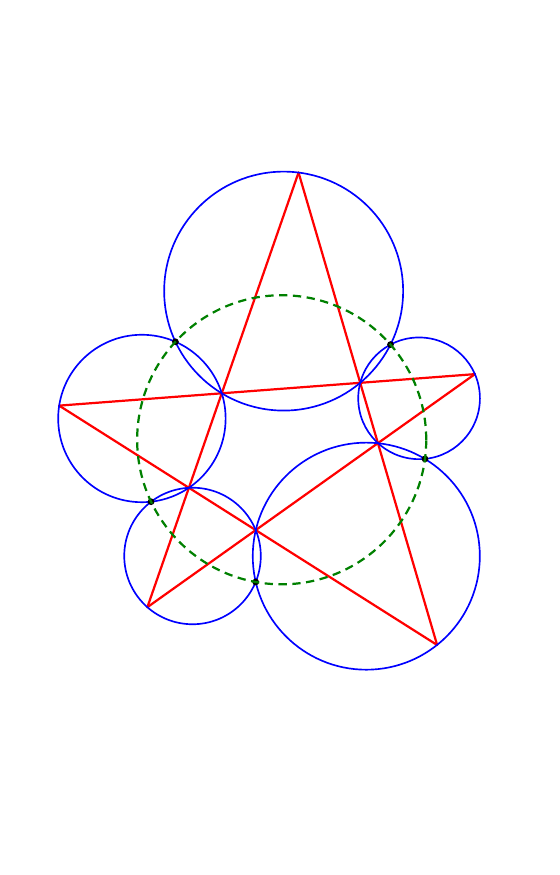
\begin{tikzpicture}[>=latex, scale=0.8]
  \useasboundingbox(-4,-6.5)rectangle(4,6.5);
  \tkzDefPoints{0.3/4.2/A,-3.5/0.5/B,-2.1/-2.7/C,2.5/-3.3/D,3.1/1.0/E}
  \tkzInterLL(A,C)(B,E)\tkzGetPoint{L}
  \tkzInterLL(A,C)(B,D)\tkzGetPoint{M}
  \tkzInterLL(B,D)(C,E)\tkzGetPoint{N}
  \tkzInterLL(C,E)(D,A)\tkzGetPoint{P}
  \tkzInterLL(D,A)(B,E)\tkzGetPoint{Q}
  \tkzDrawSegments[red,thick](A,C B,D C,E A,D B,E)
  \foreach \x/\y/\z [count=\i] in {A/L/Q,B/L/M,C/M/N,D/N/P,E/Q/P}
  {
    \tkzDefCircle(\x,\y,\z) \tkzGetPoint{O\i}
    \tkzDrawCircle[blue,semithick](O\i,\x)
  }
  \tkzInterCC(O1,A)(O2,B)\tkzGetPoints{L''}{L'}
  \tkzInterCC(O2,B)(O3,C)\tkzGetPoints{M''}{M'}
  \tkzInterCC(O3,C)(O4,D)\tkzGetPoints{N''}{N'}
  \tkzInterCC(O4,D)(O5,E)\tkzGetPoints{P''}{P'}
  \tkzInterCC(O5,E)(O1,A)\tkzGetPoints{Q''}{Q'}
  \tkzDrawPoints[fill=black](L',M',N',P',Q')
  \tkzDefCircle(L',M',N')\tkzGetPoint{O}
  \tkzDrawCircle[green!50!black,densely dashed,thick](O,N')
\end{tikzpicture}
\end{document}